\subsection{Pixel size, magnification and resolution}
Our result from calculating how many pixels in the image (see figure \ref{fig:TestChart}) that corresponds to one centimetre were 41. When we calculated the length of a car in the image (see figure \ref{fig:Toy1}) we got the result 10 cm. When comparing the resolution from two images (see figure \ref{fig:Toy1} and \ref{fig:Toy2}) of a object at different distances, we got the result of more pixels per cm when closer to the object.

\begin{figure}[h]
	\centering
	\begin{subfigure}[b]{0.3\textwidth}
		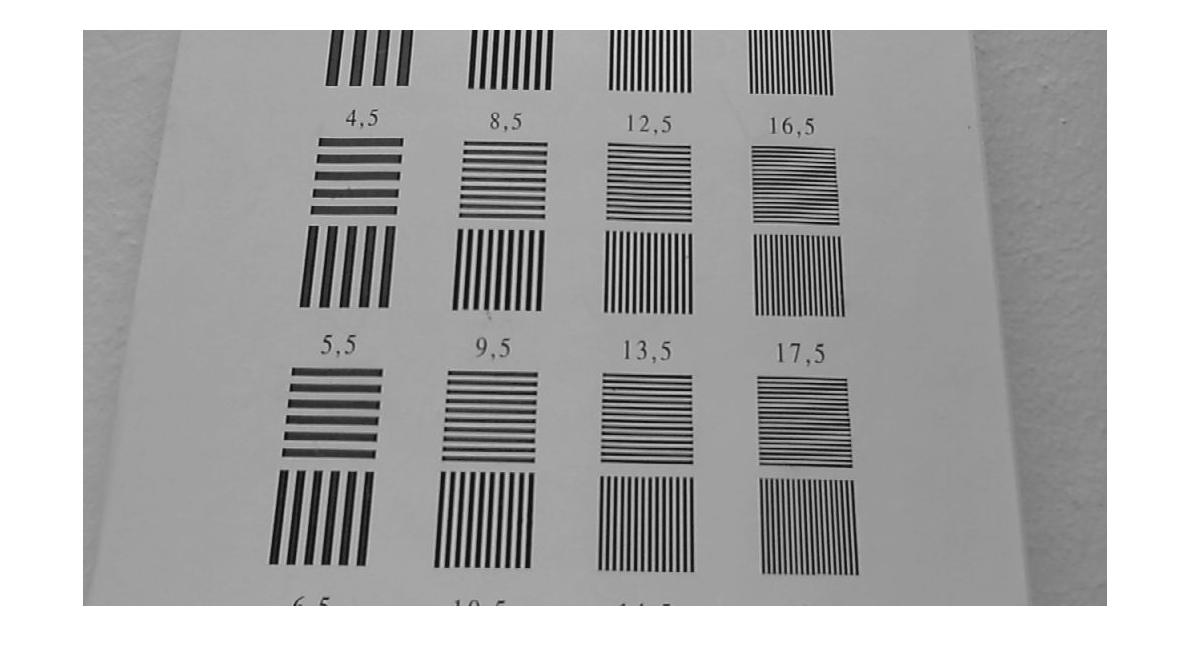
\includegraphics[width=\textwidth]{part1image1}
		\caption{}
		\label{fig:TestChart}
	\end{subfigure}
	\begin{subfigure}[b]{0.3\textwidth}
		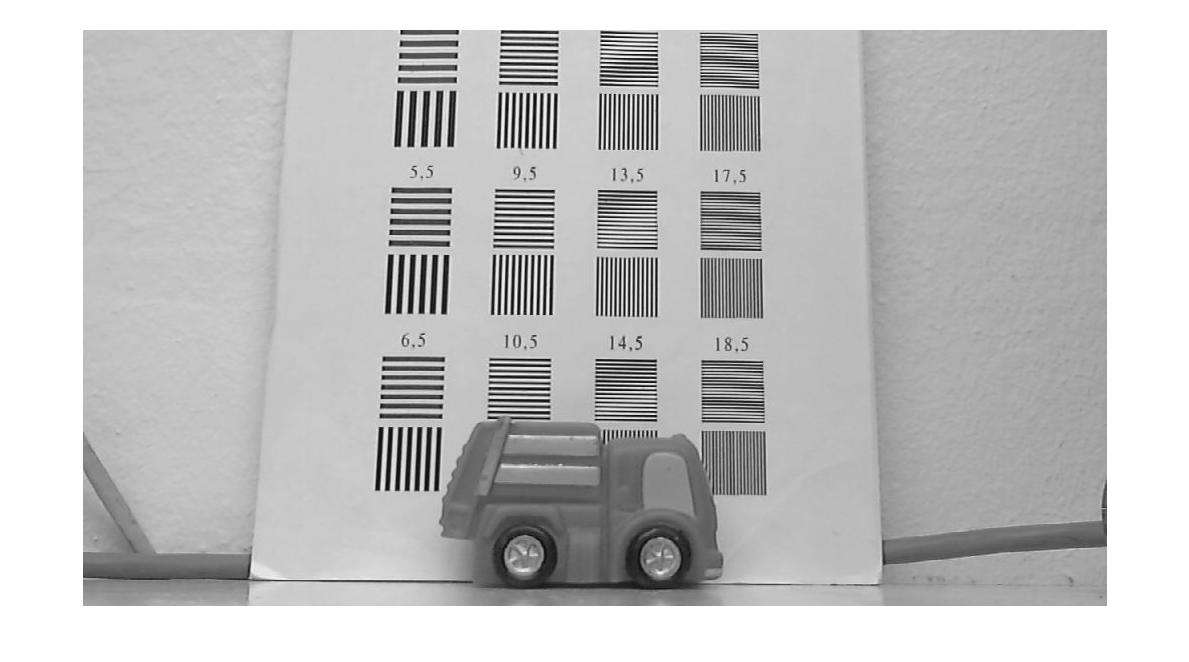
\includegraphics[width=\textwidth]{leksak1}
		\caption{}
		\label{fig:Toy1}
	\end{subfigure}
	\begin{subfigure}[b]{0.3\textwidth}
		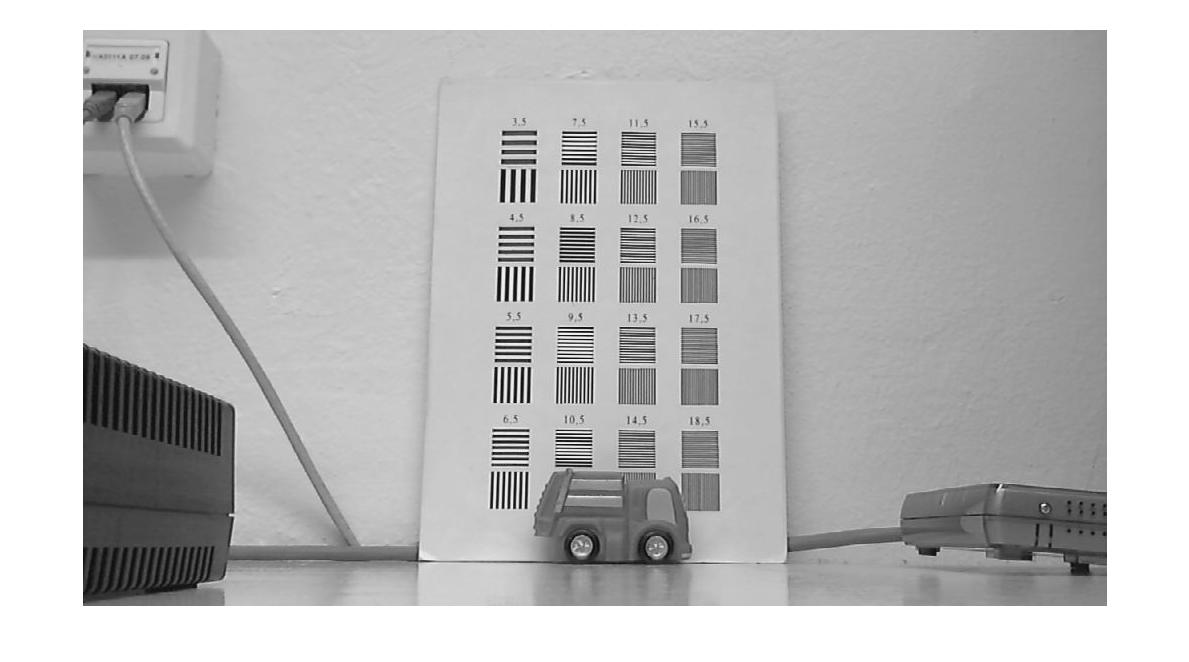
\includegraphics[width=\textwidth]{leksak2}
		\caption{}
		\label{fig:Toy2}
	\end{subfigure}
	\caption{(a) Image of test chart used to calculate how many pixels correspond to 1 cm. (b) Image used to measure distance of object and to compare the vertical and horizontal . (c) Image used to compare the resolution for different distances.}
	\label{fig:part1}
\end{figure}

\subsection{Grey scale images, image format and image information}
The function mesh shows different depths depending on what colour the pixels have (see figure \ref{fig:meshCar}), the function surfl --->What does it really do?<------ (see figure \ref{fig:surflCar}), the functions flipud and fliplr flips the image vertically and horizontally respectively. 

The result of taking the matrix I2 and subtract with I1 we get an almost black image with the edges from the car (see figure \ref{fig:I2_I1})

The MTF-values for the whole image system is shown in figure \ref{fig:mtf}

\begin{figure}[h]
\centering
	\begin{subfigure}[b]{0.4\textwidth}
		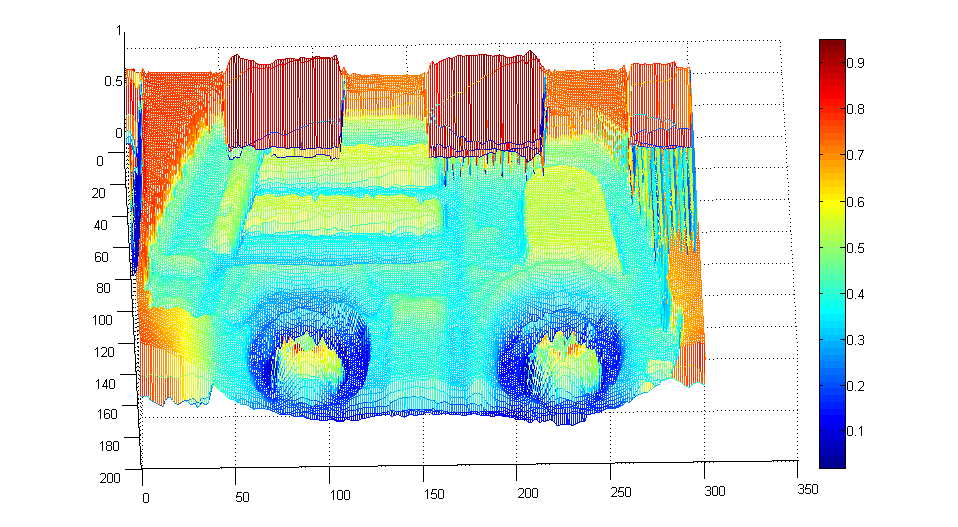
\includegraphics[width=\textwidth]{part2_mesh_croppedCar2}
		\caption{}
		\label{fig:meshCar}
	\end{subfigure}
	\begin{subfigure}[b]{0.4\textwidth}	
		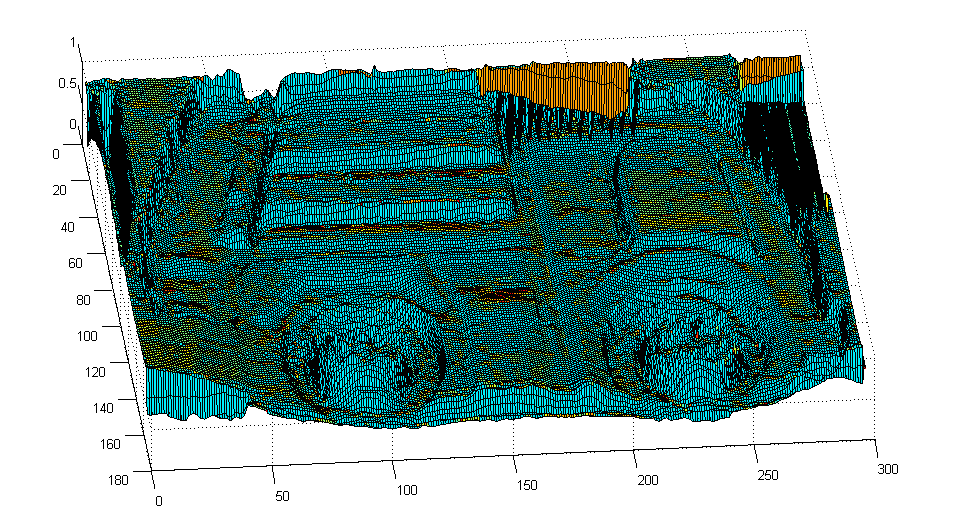
\includegraphics[width=\textwidth]{part2_surfl_croppedCar}
		\caption{}
		\label{fig:surflCar}
	\end{subfigure}
	\caption{(a) Matlab function mesh used on the cropped car image. (b) Matlab function surfl used on the cropped car image. }
	\label{fig:part2}
\end{figure}
\begin{figure}[h]
	\centering
	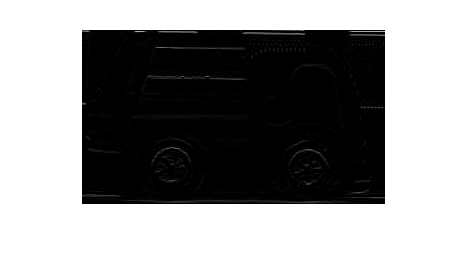
\includegraphics[width=0.5\textwidth]{part2_I1_I2}
	\caption{Subtracting a matrix with it self after shifted 1 pixel}
	\label{fig:I2_I1}
\end{figure}
\begin{figure}[h]
	\centering
	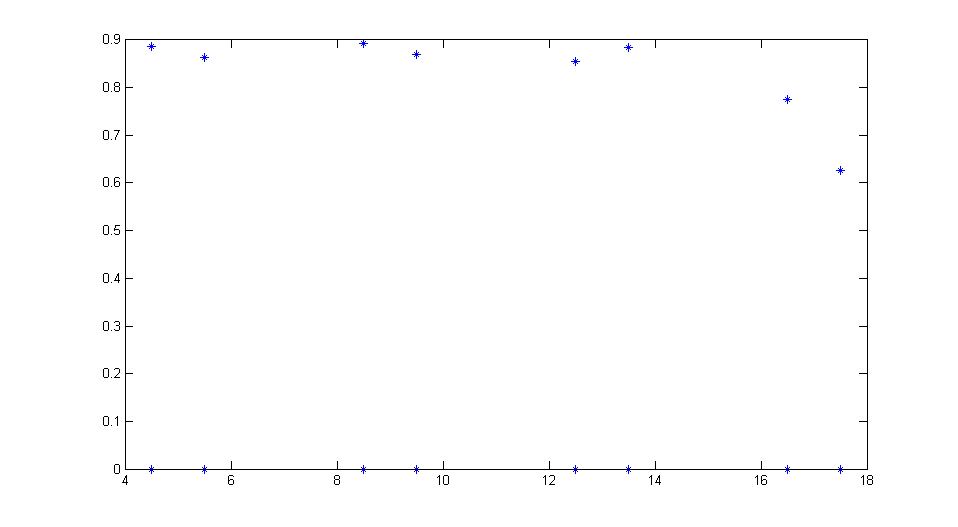
\includegraphics[width=0.5\textwidth]{part2_mtfdiagram}
	\caption{MTF-diagram for the image}
	\label{fig:mtf}
\end{figure}

\subsection{Image enhancement}
The results for image enhancement is seen in figure \ref{fig:img1new} and \ref{fig:img2new} the corresponding histogram is seen in figure \ref{fig:img1histnew} and \ref{fig:img2histnew}. The original images and there histograms can also be found in image \ref{fig:img1} and \ref{fig:img2}.
\begin{figure}[h]
	\centering
	\begin{subfigure}[b]{0.4\textwidth}
		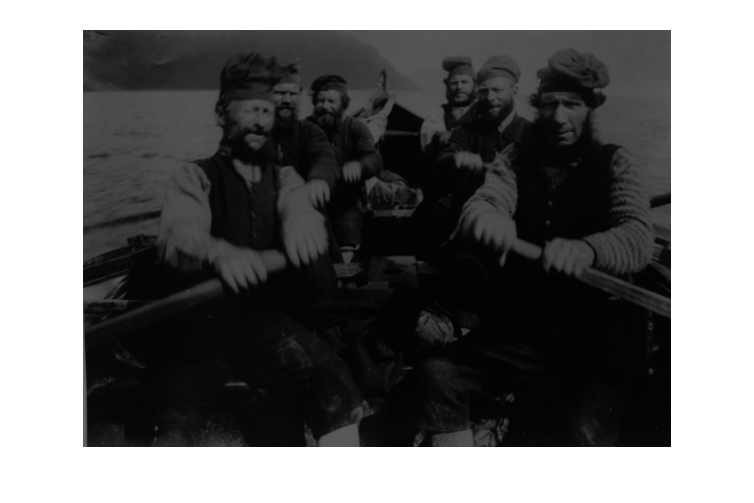
\includegraphics[width=\textwidth]{IE_img1org}
		\caption{}
		\label{fig:img1org}
	\end{subfigure}
	\begin{subfigure}[b]{0.4\textwidth}
		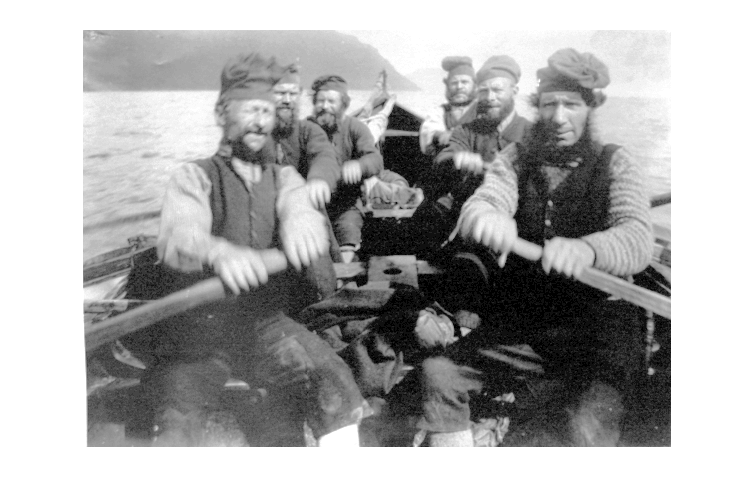
\includegraphics[width=\textwidth]{IE_img1New}
		\caption{}
		\label{fig:img1new}
	\end{subfigure}
	\\
	\begin{subfigure}[b]{0.4\textwidth}
		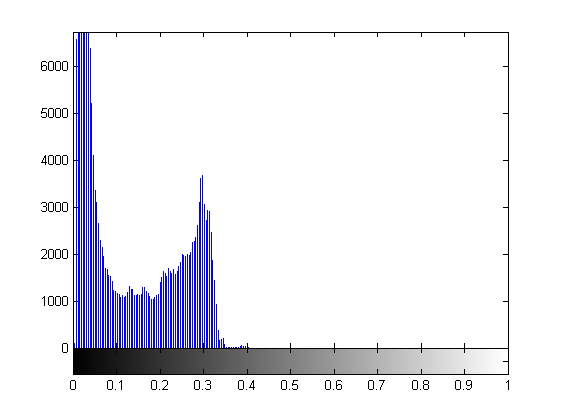
\includegraphics[width=\textwidth]{IE_img1_histOrg}
		\caption{}
		\label{fig:img1historg}
	\end{subfigure}
	\begin{subfigure}[b]{0.4\textwidth}
		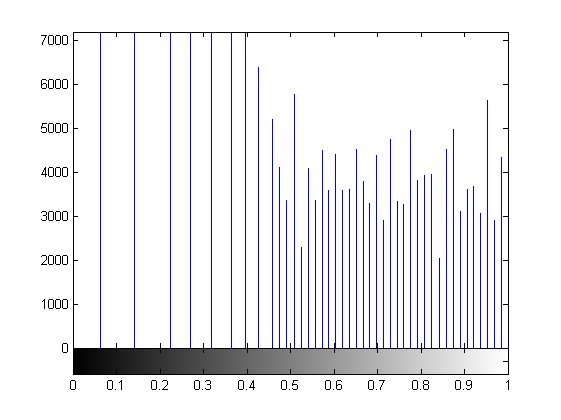
\includegraphics[width=\textwidth]{IE_img1_histNew}
		\caption{}
		\label{fig:img1histnew}
	\end{subfigure}
	\caption{(a) Original image. (b) Enhanced image. (c) Histogram for original image. (d) Histogram for enhanced image.}
	\label{fig:img1}
\end{figure}
\begin{figure}[h]
	\centering
	\begin{subfigure}[b]{0.4\textwidth}
		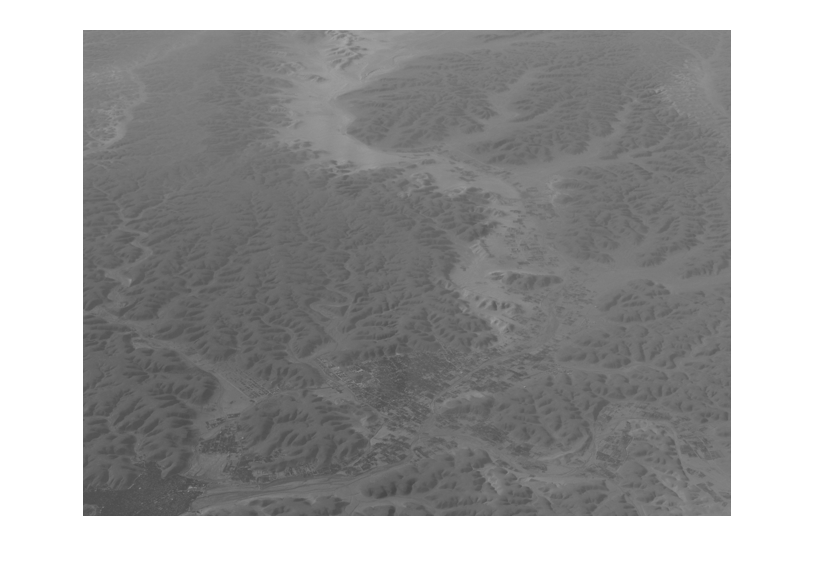
\includegraphics[width=\textwidth]{IE_img2org}
		\caption{}
		\label{fig:img2org}
	\end{subfigure}
	\begin{subfigure}[b]{0.4\textwidth}
		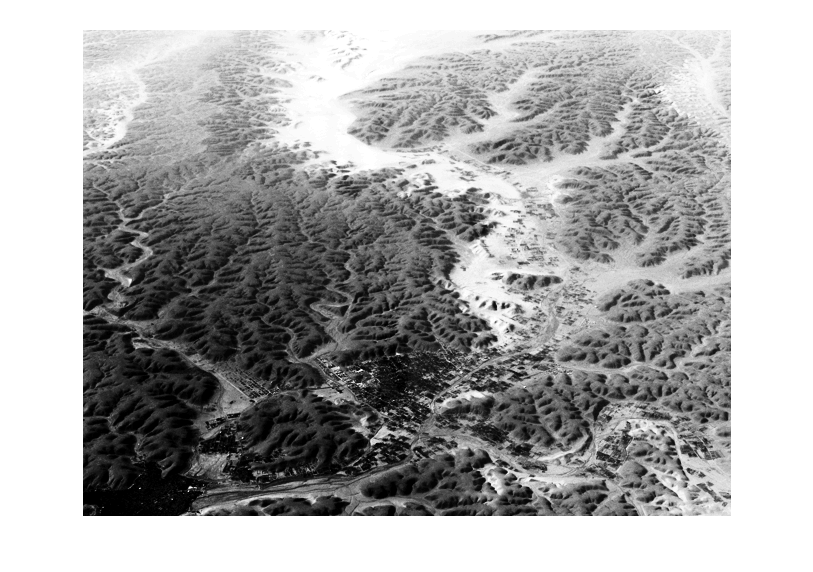
\includegraphics[width=\textwidth]{IE_img2New}
		\caption{}
		\label{fig:img2new}
	\end{subfigure}
	\\
	\begin{subfigure}[b]{0.4\textwidth}
		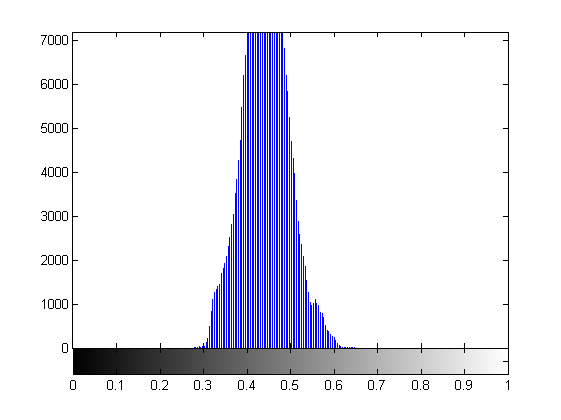
\includegraphics[width=\textwidth]{IE_img2_histOrg}
		\caption{}
		\label{fig:img2historg}
	\end{subfigure}
	\begin{subfigure}[b]{0.4\textwidth}
		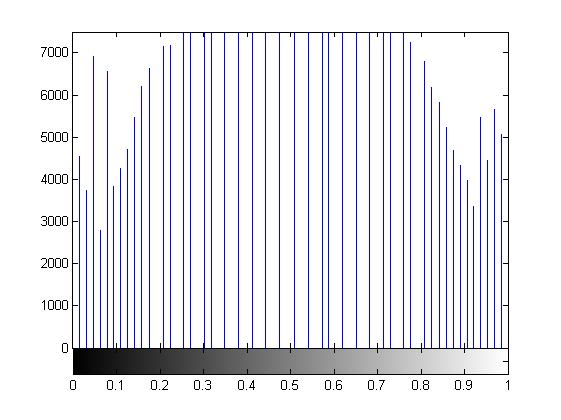
\includegraphics[width=\textwidth]{IE_img2_histNew}
		\caption{}
		\label{fig:img2histnew}
	\end{subfigure}
	\caption{(a) Original image. (b) Enhanced image. (c) Histogram for original image. (d) Histogram for enhanced image.}
	\label{fig:img2}
\end{figure}

\subsection{Colour images}
\begin{figure}[h]
	\centering
	\begin{subfigure}[b]{0.4\textwidth}
		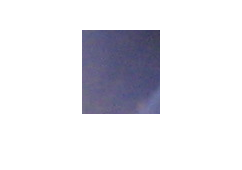
\includegraphics[width=\textwidth]{part4_bluecarcrop}
		\caption{A cropped blue part of a car}
		\label{fig:blueCrop}
	\end{subfigure}
	\begin{subfigure}[b]{0.4\textwidth}
		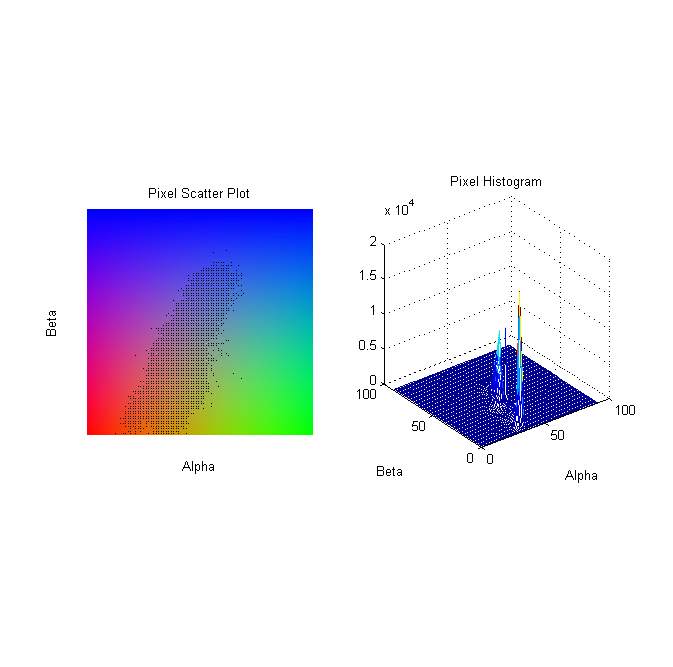
\includegraphics[width=\textwidth]{part4_anghist2_bluecar}
		\caption{Histogram on the blue part}
		\label{fig:blueSpec}
	\end{subfigure}
	\\
	\begin{subfigure}[b]{0.4\textwidth}
		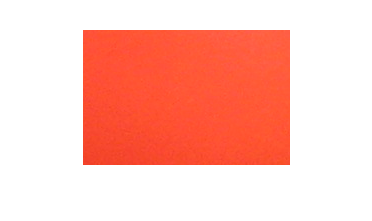
\includegraphics[width=\textwidth]{part4_smallredcrop}
		\caption{A cropped red part of a car}
		\label{fig:redCrop}
	\end{subfigure}
	\begin{subfigure}[b]{0.4\textwidth}
		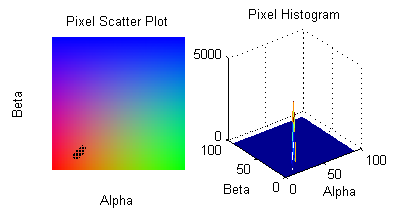
\includegraphics[width=\textwidth]{part4_anghist2_redcar}
		\caption{Histogram on the red part}
		\label{fig:redSpec}
	\end{subfigure}
	\caption{Histogram using function \texttt{anghist2}}
	\label{fig:img1}
\end{figure}

\subsection{IR - Imaging}